% ============================================================
% AUTH
% ============================================================

\subsection*{Weak Password Recovery Mechanism via Security Question (AUTH)}

\begin{table}[H]
\centering
\begin{tabular}{|l|p{10cm}|}
\hline
\textbf{Finding ID} & AUTH \\
\hline
\textbf{Severity} & Critical \\
\hline
\textbf{CVSS 3.1 Score} & 9.1 (Critical) \\
\hline
\textbf{CVSS Vector} & \texttt{AV:N/AC:L/PR:N/UI:N/S:U/C:H/I:H/A:N} \\
\hline
\textbf{Status} & Confirmed \\
\hline
\textbf{OWASP Category} & A07:2021 -- Identification and Authentication Failures \\
\hline
\textbf{CWE} & CWE-640 -- Weak Password Recovery Mechanism for Forgotten Password \\
\hline
\textbf{Affected Functionality} & Forgot Password / Password Recovery \\
\hline
\textbf{Affected Account} & \texttt{jim@juice-sh.op} \\
\hline
\end{tabular}
\caption{Weak Password Recovery Mechanism finding details}
\end{table}

\subsubsection*{Description}

The password recovery functionality was found to rely on a security
question whose answer could be discovered or guessed using publicly
available information.

The application allows a user who provides the correct answer to the
security question to set a new password for the target account.

During testing, the security question for the account
\texttt{jim@juice-sh.op} was:

\begin{lstlisting}
Your eldest siblings middle name?
\end{lstlisting}

The answer was identified as \texttt{Samuel} based on publicly
available information associated with the account's identity.

After submitting the correct answer, the application allowed a new
password to be set successfully.

This demonstrates that the password recovery mechanism does not
provide sufficiently strong proof of account ownership.

\subsubsection*{Methodology}

The Forgot Password functionality was tested manually.

The password recovery process was initiated for the target account.
The security question displayed by the application was reviewed.

The answer was then identified using publicly available information
related to the target account.

The identified answer was submitted to the password recovery form.
The application accepted the answer and allowed a new password to be
created.

The successful password reset was used as evidence that the recovery
mechanism could be bypassed without knowledge of the original
password.

\subsubsection*{Steps to Reproduce}

\begin{enumerate}

    \item Open the Forgot Password functionality:

    \begin{lstlisting}
http://127.0.0.1:3000/#/forgot-password
    \end{lstlisting}

    \item Enter the target email address:

    \begin{lstlisting}
jim@juice-sh.op
    \end{lstlisting}

    \item Observe the security question:

    \begin{lstlisting}
Your eldest siblings middle name?
    \end{lstlisting}

    \item Identify the answer using publicly available information
    associated with the target account.

    \item Enter the answer:

    \begin{lstlisting}
Samuel
    \end{lstlisting}

    \item Enter a new password and confirm the new password.

    \item Submit the password reset form.

    \item Observe that the application confirms that the password was
    successfully changed.

\end{enumerate}

\subsubsection*{Evidence}

The following evidence demonstrates the weak security-question
mechanism and successful password reset.

\begin{figure}[H]
    \centering
    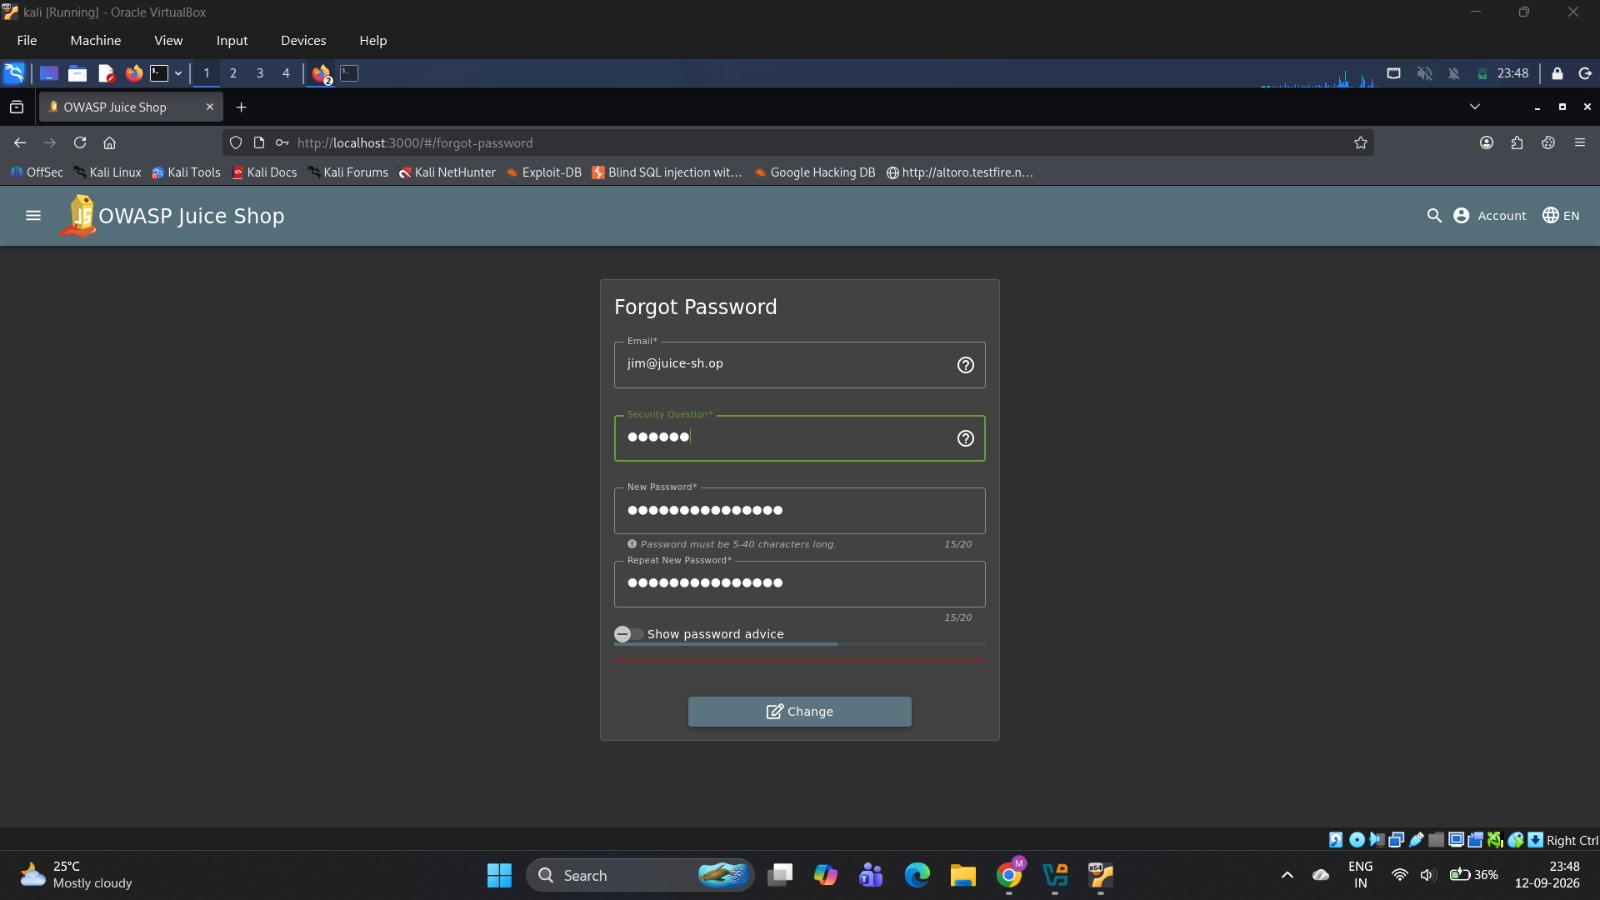
\includegraphics[width=0.8\textwidth]
    {evidence/phase4/authentication/01_forgot_password_security_answer.jpg}
    \caption{Forgot Password process with the security question answered}
\end{figure}

\begin{figure}[H]
    \centering
    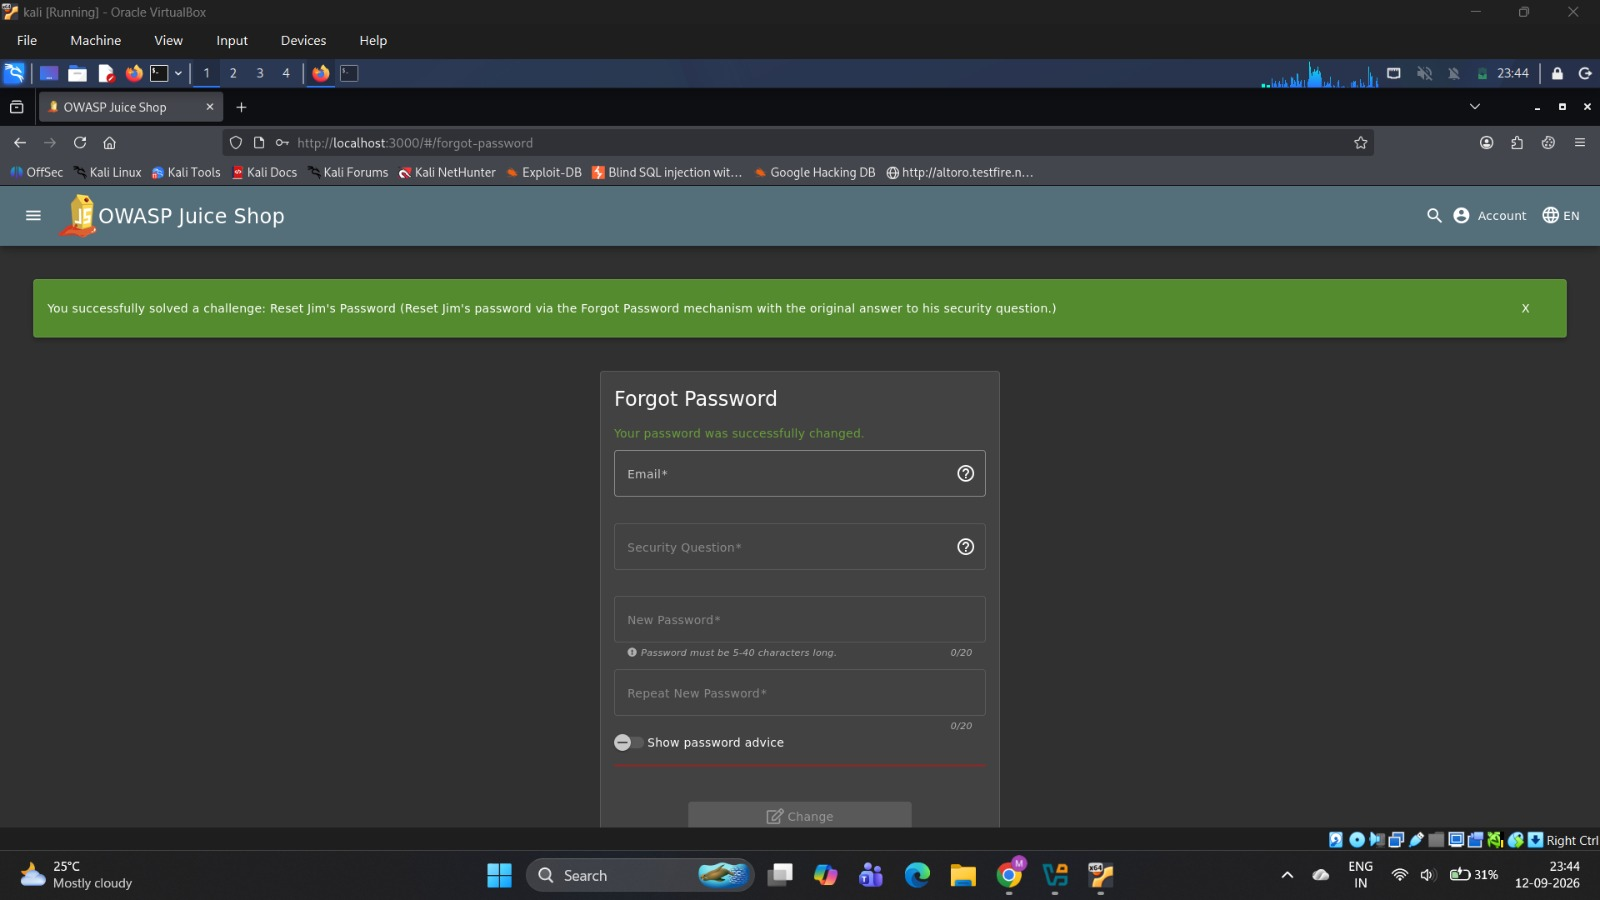
\includegraphics[width=0.8\textwidth]
    {evidence/phase4/authentication/02_password_reset_success.jpg}
    \caption{Application confirming that the password was successfully changed}
\end{figure}

\subsubsection*{Impact}

An attacker who can discover or guess the answer to the security
question may be able to reset the victim's password without knowing
the original password.

This can result in unauthorized access to the affected account and
may lead to account takeover.

The impact may be greater if the affected account has access to
sensitive information or privileged functionality.

\subsubsection*{Remediation}

\begin{itemize}

    \item Do not rely on easily discoverable security questions as the
    primary mechanism for password recovery.

    \item Use a secure password-reset mechanism based on a
    cryptographically random, single-use, time-limited reset token.

    \item Send password-reset links or verification codes through a
    previously verified communication channel.

    \item Expire password-reset tokens after a short period and
    invalidate them after successful use.

    \item Apply rate limiting and monitoring to password-recovery
    attempts.

    \item Do not reveal sensitive information that helps an attacker
    determine whether a target account exists.

\end{itemize}

\subsubsection*{Conclusion}

The weak password recovery mechanism was successfully confirmed
through manual testing.

The application accepted an answer to a predictable security
question and allowed a new password to be set for the target account
without requiring the original password.

The finding is therefore classified as a confirmed Critical-severity
Identification and Authentication Failure.